\qrchapter{https://forgottenpillar.com/rsc/sw-fp-chapter10}{Je, Mungu ni nafsi? - na John N. Loughborough}

Mojawapo ya makala ya mapema zaidi juu ya \emcap{Umbile la Mungu} ni nakala ya Loughborough “\textit{Je, Mungu ni nafsi?}” ambapo anazungumzia \emcap{Umbile la Mungu} na uwepo wake. Ni muhimu kumbuka maana ya ‘personality’ kulingana na kamusi ya Merriam-Webster: “\textit{Ubora au hali ya kuwa Nafsi}”\footnote{\href{https://www.merriam-webster.com/dictionary/personality}{Merriam-Webster Dictionary - ‘\textit{personality}’}}. Tutaangalia kwa uangalifu jinsi Loughborough anavyoona ubora au hali ya Mungu kuwa Nafsi.

\begin{figure}[hp]
    \centering
    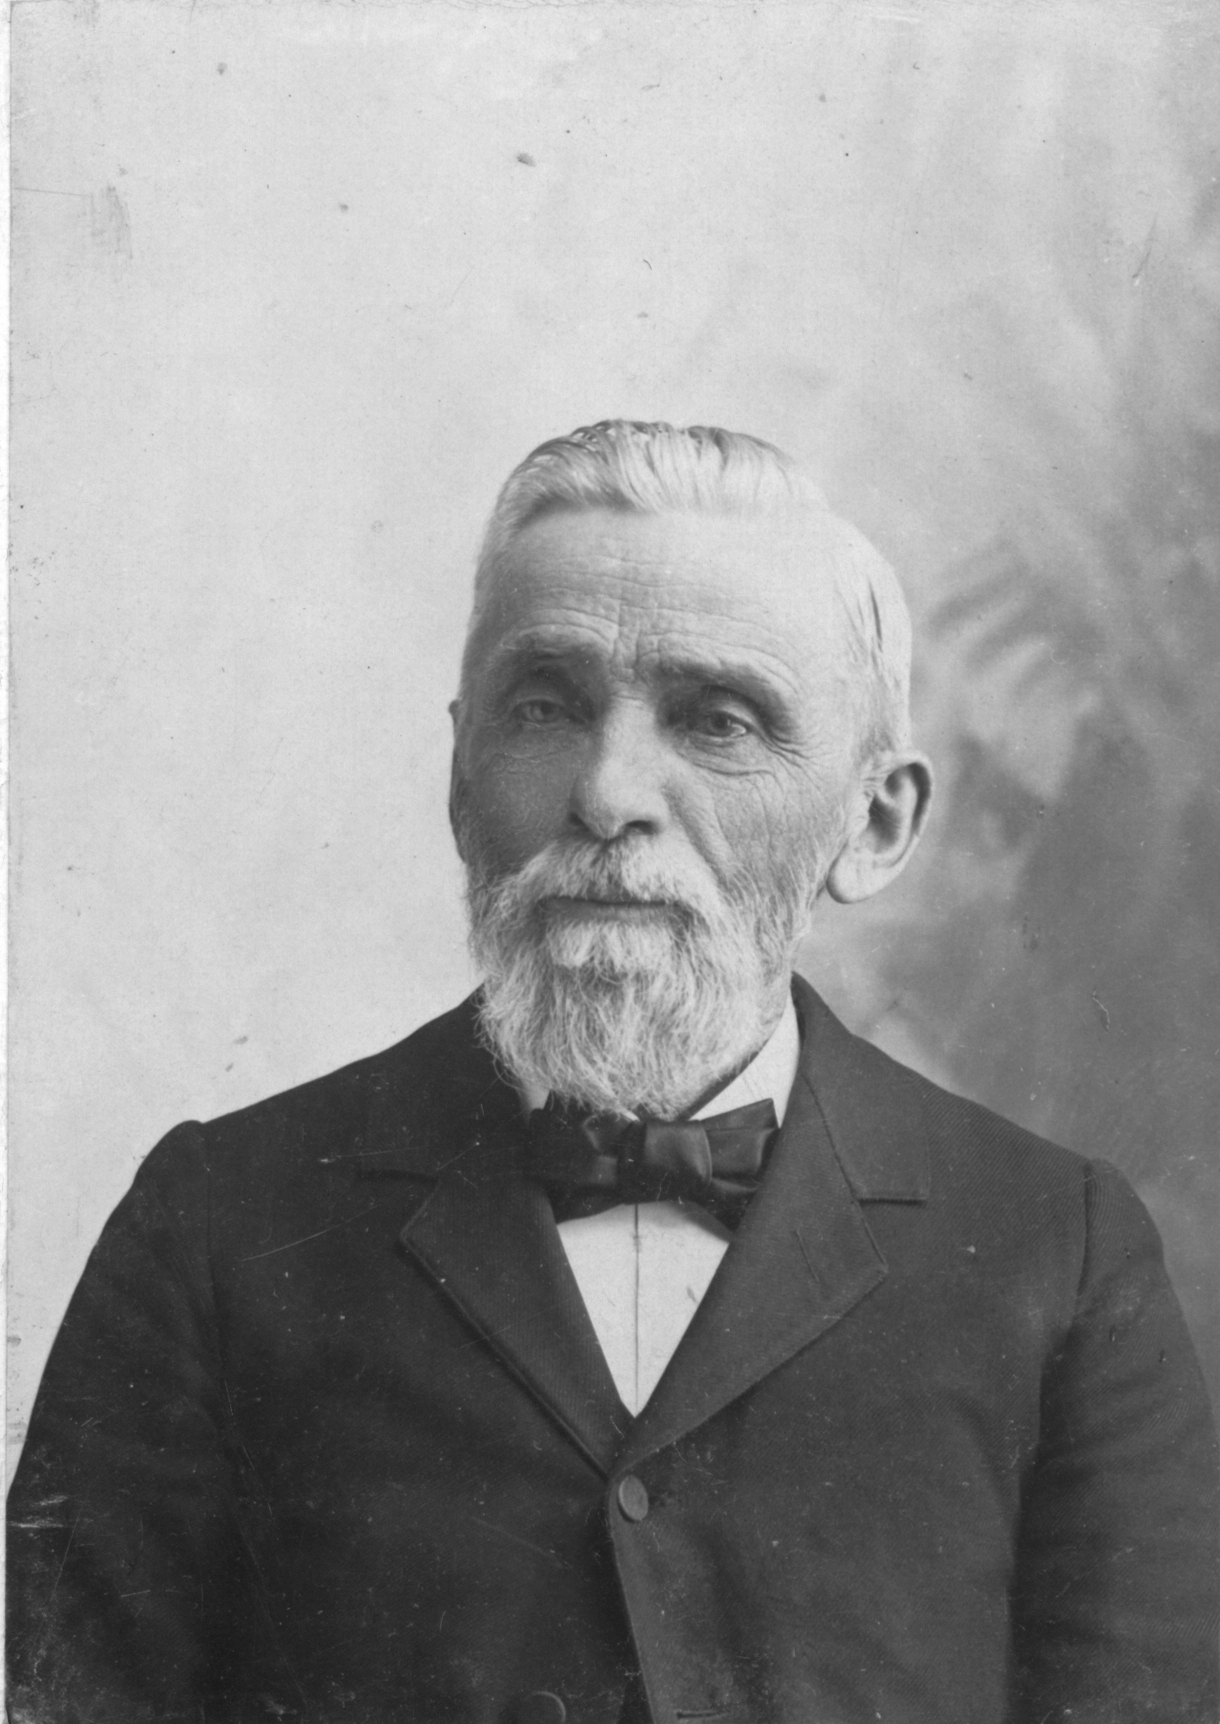
\includegraphics[width=1\linewidth]{images/john-n-loughborough.jpg}
    \caption*{John Norton Loughborough (1832-1924)}
    \label{fig:john-n-loughborough}
\end{figure}

\others{Chochote kinachoweza kuwa ukweli katika suala hili, hakika haiwezi kuwa vibaya kwetu kuchunguza kile ambacho Neno linasema juu yake. \textbf{Kuna wengi ambao wangejiepusha na uchunguzi wa ukweli usiopendwa na watu wengi kwa sababu kilio cha uzushi kinainuliwa dhidi yao}. Sisi hatutajiona kuwa watu wa jina hilo, \textbf{wala hatujiingizi ndani ya siri za Mwenyezi, tunapofuatilia uchunguzi wa jambo hili}. Bibilia hakika ina ushuhuda juu ya jambo hili, na tunarudia tena, ‘\textbf{Vitu vilivyofunuliwa kwetu ni vyetu}.’ Tunauliza basi, Maandiko Matakatifu yasemaje?}

\othersnogap{\textbf{Ushuhuda wenyewe ambao tumekuwa tukichunguza kuhusu mwanadamu kuumbwa kwa mavumbi \underline{katika mfano wa Mungu}, unathibitisha kabisa kwamba \underline{Mungu ana fomu}, ingawa hisia hii ni kinyume na yale tumefundishwa, tulipokuwa watoto, kutoka katekisimu}:}

\othersnogap{Swali. ‘Mungu ni nini?’}

\othersnogap{Jibu. ‘Roho isiyo na mwisho na ya milele; moja ambayo sikuzote ilikuwako na itakuwako daima.’}

\othersnogap{Swali. ‘Mungu yuko wapi?’}

\othersnogap{Jibu. ‘Kila mahali.’}

\othersnogap{Tunajibu, \textbf{somo limeanzishwa katika mstari wa 7, kama ifuatavyo}: ‘\textbf{\underline{Nitaenda wapi kutoka kwa Roho yako}?} \textbf{au nitakimbilia wapi kutoka kwa \underline{uwepo wako}?}’ \textbf{Roho ni \underline{mwakilishi wa Mungu}}. \textbf{Nguvu zake hudhihirika popote anapotaka, kupitia wakala wa Roho wake}. Kristo, anapowapa wanafunzi agizo, anasema, ‘Enendeni ulimwenguni mwote, mkahubiri Injili kwa kila kiumbe, na hakika! \textbf{Niko pamoja nanyi siku zote, hata hadi mwisho wa dahari}.’ Sasa, hakuna mtu ambaye angepinga kwamba Kristo amekuwa duniani kibinafsi tangu wakati wanafunzi wake walianza kutimiza agizo hili. \textbf{Lakini Roho wake amekuwa juu ya nchi; Mfariji ambaye aliahidi kutuma.} \textbf{Hivyo kwa namna hiyo hiyo Mungu hujidhihirisha \underline{kupitia kwa Roho yake} ambayo pia ni nguvu ambayo kwayo anafanya kazi}. ‘Lakini ikiwa \textbf{Roho wa huyo} aliyemfufua Yesu kutoka kwa wafu atakaa ndani yenu, \textbf{yeye aliyemfufua Kristo} kutoka kwa wafu atahuisha miili yenu iliyo katika hali ya kufa \textbf{\underline{kwa Roho wake} akaaye ndani yenu}.’ Warumi 8:11. \textbf{\underline{Hapa kuna utofauti wa wazi kati ya Roho, na Mungu ambaye huwafufua wafu kwa Roho huyo}}. \textbf{Ikiwa Mungu aliye hai ni Roho kwa maana kali ya neno, na wakati huo huo anamiliki Roho, basi tunapata wazo jipya la Roho wa Roho, jambo ambalo litamhitaji angalau Mmizimu kueleza}.}[The Adventist Review and Sabbath Herald, September 18, 1855][https://documents.adventistarchives.org/Periodicals/RH/RH18550918-V07-06.pdf]

Turuhusu tutoe maoni mafupi. Tunatumahi unatambua mada mahususi inayojadiliwa hapa. Somo ni hoja ya kwanza ya \emcap{Kanuni za Msingi} na madai ni kwamba Mungu ana fomu, kwa maana mwanadamu ameumbwa kwa mfano wa Mungu. Uelewa kama huo wa ubinafsi wa Mungu huzuia wazo la kwamba Mungu yuko kila mahali. Ndugu Loughborough alitoa sababu za kibiblia za uwepo wa Mungu kila mahali, pamoja na maoni kwamba “\textit{Mungu yuko katika sehemu moja zaidi ya nyingine}”. Mungu yuko kila mahali kupitia kwa mwakilishi wake, Roho Mtakatifu, kama ilivyoandikwa katika hoja ya kwanza ya \emcap{Kanuni za Msingi}. Zaidi katika majadiliano haya, tutasoma kwamba Mungu ni huluki ya kiroho na anamiliki mwili unaoonekana na kushikika, tofauti na wazo kwamba Yeye ni roho tu.

\others{Kuna angalau ugumu mmoja usiopitika katika njia ya \textbf{wale wanaomwamini \underline{Mungu anakosa mwili}, na mbingu si mahali halisi, panapo-dhihirika: wanalazimika kukubali kwamba \underline{Yesu yuko pale kimwili, nafsi halisi}}; Yesu yule yule aliyesulubiwa, akafa, na akazikwa, akafufuliwa kutoka kwa wafu, \textbf{akapaa juu mbinguni}, na sasa yuko \textbf{upande wa mkono wa kuume wa Mungu}. \textbf{Yesu alimiliki nyama na mifupa baada ya kufufuka kwake}. Luka 24:39. ‘\textbf{Tazameni mikono yangu na miguu yangu, ya kuwa ni mimi mwenyewe; nishikeni, mwone; \underline{kwa maana roho haina nyama na mifupa kama mnionavyo kuwa nayo}}.’ \textbf{Ikiwa Yesu yuko mbinguni akiwa na mwili halisi ya nyama na mifupa,isiwezekane mbinguni iwe mahali halisi, makao ya halisi Mungu, Mwokozi halisi, malaika halisi, na watakatifu waliofufuliwa wasioweza kufa?} \textbf{\underline{Hapana, anasema moja, ‘Mungu ni Roho.’}} Ndivyo Kristo alimwambia mwanamke Msamaria kwenye kisima. \textbf{Haifuatii kwa ulazima eti kwa sababu Mungu ni Roho, \underline{kwamba hana mwili}}. Katika Yohana 3:6, Kristo anamwambia Nikodemo, ‘\textbf{Kilichozaliwa kwa Roho ni roho}.’ \textbf{Ikiwa kile kilichozaliwa na Roho ni roho, basi kwa kanuni hiyo hiyo, kilicho na asili ya kiroho ni roho. Mungu ni \underline{huluki roho}, asili yake ni roho, yeye si wa mwili wa kufa; }\textbf{\underline{lakini hii haiondoi wazo la yeye kuwa na mwili}}. Daudi asema, [Zaburi 114:4,] ‘Ni nani afanyaye \textbf{malaika wake roho};’ bado \textbf{\underline{malaika wana miili}}. Malaika waliwatokea Ibrahimu na Lutu, na wakakula nao. \textbf{Tunaona wazo la kwamba malaika ni roho, halithibitishi kwamba si viumbe halisi}.}

\othersnogap{Imefikiriwa kwa sababu Biblia inasema kwamba Mungu ni Roho, eti yeye si nafsi. Mtazamo haupaswi kuwa msingi wa hoja. Kweli kuu za Maandiko zinasemwa wazi, na haitatufanyia kuunda fundisho juu ya makisio, \textbf{kinyume na kauli chanya katika neno la Mungu}. Ikiwa Maandiko yanasema kwa maneno chanya \textbf{kwamba Mungu ni nafsi, haitakuwa jibu kwetu kuchukua hitimisho kutoka kwa kifungu kinachosema ‘Mungu ni Roho,’ \underline{kwamba yeye hana mwili}}.}

\othersnogap{Sasa tutawasilisha vifungu vichache \textbf{vinavyothibitisha kwamba Mungu ni nafsi}. Kutoka 33:18, 23. ‘Na yeye (Musa) akasema, nakuomba unionyeshe utukufu wako.’ Aya 20. ‘Na akamwambia, \textbf{Huwezi ona \underline{uso wangu}, kwa maana hakuna mtu atakayeniona na kuishi}.’ Mstari wa 21-23. ‘Bwana akasema, Tazama, kuna mahali karibu nami, nawe utasimama juu ya mwamba: na itatimia wakati utukufu wangu utapita, nitakuweka katika ufa wa mwamba; na \textbf{nitakufunika na \underline{mkono wangu} nipitapo}; nami nitauondoa \textbf{mkono wangu}, nawe utaniona \textbf{sehemu zangu za \underline{nyuma}}; lakini \textbf{\underline{uso wangu} hautaonekana.’} \textbf{Ikiwa Mungu ni \underline{Roho asiye na mwili}, basi Musa asingeweza kumwona; kwa maana tunaambiwa roho haiwezi kuonekana kwa macho ya kawaida}. \textbf{Basi Mungu asingekuwa mwenye haki kusema kwamba angeweka mkono wake juu ya uso wa Musa wakati yeye angepita (ikionekana kumzuia asiuone uso wake), kwa maana hakuweza kumwona}. Wala hatufikirii jinsi mkono usio na mwili unavyoweza kuzuia miale ya mwanga kupita kwa macho ya Musa. \textbf{Lakini ikiwa msimamo huo ni wa kweli \underline{kwamba Mungu hana mwili}, na hawezi kuonekana kwa jicho la kawaida, maandishi ya hapo juu yote ni yasiyohitajiwa}. \textbf{Kuna maana gani ya kusema Mungu akaweka mkono wake juu ya uso wa Musa, ili kumzuia asione kile ambacho hakiwezi kuonekana}.}

\othersnogap{Anasema mmoja, naona hatuwezi kuoanisha jambo hilo kwa njia nyingine yoyote, isipokuwa kwamba kulikuwa na mwili halisi ulioonekana na Musa; lakini huo haukuwa mwili wa Mungu mwenyewe, \textbf{bali ni mwili alioutwaa ili aweze kujionyesha kwa Musa}. \textbf{Musa hakuweza kuunda dhana za haki za Mungu isipokuwa tu akichukua fomu.} \textbf{Kwa hiyo Mungu akatwaa mwili}. Hii inatupa rangi mbaya zaidi juu ya jambo hilo kuliko nafasi iliyotolewa ya kwanza; \textbf{kwa maana inamsingizia Mungu udanganyifu; kumwambia Musa amwone, wakati kwa hakika Musa kulingana na ushuhuda huu hakuona Mungu, bali mwili mwingine}. Mtu lazima apeanwe kwa shaka karibu zaidi ya kupona, ambayo ingejaribu kuficha, na kuondoa nguvu ya ushuhuda huu.}[Ibid.][https://documents.adventistarchives.org/Periodicals/RH/RH18550918-V07-06.pdf]

Je, unatambua kwamba Ndugu Loughborough anashughulikia hisia ambazo Dk. Kellogg angewasilisha katika Hekalu Hai miaka 48 baadaye? Dk. Kellogg alisema kwamba ni kweli kwamba Mungu alijidhihirisha katika\others{\textbf{\underline{namna au mahali maalum}}}[Dr. John H. Kellogg, The Living Temple, p.31.][https://archive.org/details/J.H.Kellogg.TheLivingTemple1903/page/n31/] kwa sababu \others{lazima kuwe na kitu kinachoshikika zaidi, \textbf{\underline{kinachozuiliwa}} zaidi, ambacho juu yake kitategemeza akili katika ibada}[bid, p.30][https://archive.org/details/J.H.Kellogg.TheLivingTemple1903/page/n30/], lakini kwamba Yeye yuko, kwa kweli,\others{\textbf{mbali zaidi ya ufahamu wetu \underline{kama ilivyo mipaka ya nafasi na wakati}}}[Ibid, p.33][https://archive.org/details/J.H.Kellogg.TheLivingTemple1903/page/n33/]. Ndugu Loughborough alipinga wazo la kwamba Mungu anajidhihirisha tu kwa mwanadamu kama huluki dhahiri, lakini kwa uhalisi, si kile anachojionyesha kuwa. Madai kama hayo\others{humshtaki Mungu kwa udanganyifu}. Ndugu Loughborough anaendelea na uthibitisho wa hakika, wa ushuhuda wa Kibiblia kwamba Mungu ni huluki mwenye mwili.

\others{Kutoka 24:9. ‘Basi wakaenda juu Musa, na Haruni, Nadabu na Abihu, na wazee sabini wa Israeli: \textbf{nao wakamwona Mungu wa Israeli}: na pale chini ya \textbf{miguu yake} palikuwa kama sakafu kazi ya samawi, na kama ilivyokuwa mwili wa mbinguni katika uangavu wake.’ Waliruhusiwa kuona \textbf{miguu yake}, lakini hakuna \textbf{mtu awezaye kuuona uso wake na kuishi}. \textbf{Hakuna \underline{jicho la mwanadamu} linaloweza kustahimili mng'ao unaong'aa wa utukufu ule wa uso wa Mungu}. Inazidi sana nuru ya jua. Kwa maana nabii asema, ‘Nuru ya mwezi itakuwa kama nuru ya jua, na mwanga wa jua utakuwa \textbf{mara saba}, kama nuru ya siku saba, katika siku hiyo Bwana afungapo jeraha la watu wake, na kuponya mapigo ya jeraha yao.’ Isaya 30:26. Bila Kujali nuru hii ya mara saba ambayo itaangaza, nabii akinena juu ya tukio hilo asema, ‘Ndipo mwezi utatahayarika, na jua litaaibika, wakati Bwana wa majeshi atatawala katika mlima Sayuni, na katika Yerusalemu, na mbele ya wazee wake kwa utukufu.’ Isaya 24:23. Ushuhuda wa Yohana ni, [Ufunuo 21:23,] ‘Na mji ule hauhitaji jua, wala mwezi, uangaze ndani yake: kwa maana \textbf{utukufu wa Mungu huutia nuru,} na nuru yake ni Mwana-Kondoo.’}

\othersnogap{\textbf{Makafiri wanadai kuwa kuna ukinzani katika ushahidi wa Musa, kwa sababu alisema: alizungumza na Mungu uso kwa uso}. \textbf{Sisi tunajibu, palikuwa na wingu baina yao}, lakini Mwenyezi Mungu alimwambia Musa, ‘\textbf{Hakuna mtu atakayeniona na kuishi}.’ Ushuhuda wa Agano Jipya na lile la Kale linauwiano juu ya somo hili. ‘Fuata amani na watu wote, na utakatifu bila hayo \textbf{hakuna mtu atakayemwona Bwana}.’ Waebrania 12:14. \textbf{Nani kwa \underline{macho ya kufa} anaweza kutazama nuru iangazayo zaidi ya mara saba ya mwangaza wa jua?} Hakika hakuna lakini watakatifu wanaweza kumwona, \textbf{hakuna ila macho yasiyoweza kufa} yangeweza kustahimili utukufu wa ule mngao. Ingawa Neno linasema hatuwezi kumwona Mungu sasa na kuishi, ahadi ni kwamba, \textbf{wenye mioyo safi watamwona}. Mathayo 5:3. ‘Heri wenye mioyo safi, \textbf{maana hao watamwona Mungu}.’ Ufu 22:4. ‘Nao \textbf{watauona uso wake}, na jina lake litakuwa katika vipaji vya nyuso zao.’}

\othersnogap{Paulo, [Wakolosai 1:15,] akinena juu ya Kristo, asema, ‘Naye ni mfano wa \textbf{Mungu asiyeonekana kwetu}, mzaliwa wa kwanza wa kila kiumbe.’ Hapa Kristo anasemwa kuwa ‘\textbf{mfano wa Mungu asiyeonekana kwetu}.’ Tayari tumeonyesha, kwamba\textbf{ Kristo ana mwili unaojumuisha dutu, mwili na mifupa; naye anasemwa kuwa}, ‘\textbf{mfano wa Mungu asiyeonekana kwetu}.’ Vema, asema mmoja, twakubali asili yake ya kimungu iko katika mfano wa Mungu. Ikiwa kwa asili yake ya kimungu unamaanisha sehemu iliyokuwepo katika utukufu pamoja na Baba kabla ya ulimwengu kuwako, twajibu, kile kilichokuwa hapo mwanzo na Mungu, (Neno,) \textbf{lilifanyika mwili, si kuja katika mwili}, au kama wengine husema, \textbf{kuvikwa na asili ya kibinadamu, lakini kufanyika mwili}. Lakini mwingine anasema, \textbf{Mungu anasemwa kuwa haonekani}. \textbf{Kwa sababu haonekani sasa, haithibitishi kwamba hataonekana kamwe}. Neno linasema, ‘Wenye moyo safi \textbf{watamwona}’. Imani iliyo tayari husema, Amina.}

\othersnogap{Ushuhuda wa Paulo katika Wafilipi 2:5, 6, unaonyesha wazi kile kinachoweza kueleweka kwa taarifa, kwamba Kristo ni mfano wa Mungu. ‘Iweni na nia iyo hiyo ndani yenu ambayo ilikuwa ndani ya Kristo Yesu: ambaye \textbf{alikuwa yuna fomu ya Mungu}, hakuona kuwa sawa na Mungu kuwa ni unyang'anyi.’ \textbf{Jinsi gani Kristo anaweza kusemwa kuwa katika namna ya Mungu, ikiwa Mungu hana namna?} Warumi 8:3. ‘Mungu akimtuma Mwana wake mwenyewe katika mfano wa mwili ulio wa dhambi.’ \textbf{Kristo yu katika namna ya Mungu, na katika namna ya kibinadamu. Hii mara moja inatufunulia mfano ya Mungu}.}

\othersnogap{\textbf{\underline{Danieli akinena juu ya Mungu, anamwita Mzee wa siku}}. Danieli 7:9. ‘Na Mzee wa Siku nyingi aliketi, \textbf{ambaye vazi lake lilikuwa jeupe kama theluji}, na \textbf{nywele za kichwa chake} kama sufu safi.’ \textbf{Nafsi husika anasemekana kuwa na kichwa, na nywele; hili hakika lisingeweza kusemwa kwake} \textbf{\underline{ikiwa hakuwa na mwili na hana fomu}}. \textbf{Lakini ushuhuda wa Paulo katika \underline{Waebrania 1:3}, unapaswa kusuluhisha kwa kila akili iliyonyooka \underline{kuhusiana na ubinafsi wa Mungu}}. Akizungumzia Kristo, anasema, ‘Ambaye kwa kuwa ni mng'ao wa utukufu wake, \textbf{na chapa dhahiri ya (Nafsi ya \underline{Baba})}.’ \textbf{Hapa basi inasemwa waziwazi \underline{Mungu ana nafsi}. Kristo ndiye chapa dhahiri ya nafsi hiyo.} Ndipo tunaweza kumwelewa Kristo pale anaposema, ‘\textbf{Yeye aliyeniona Mimi amemwona baba yangu}.’ Yoh. 14:19. \textbf{Hakuweza kumaanisha, kwamba alikuwa baba yake mwenyewe; kwa kuwa alipoomba alimwambia Baba yake kama mtu mwingine aliyemtuma ndani ya dunia}. Alijiita \textbf{Mwana wa Mungu}. \textbf{Basi asingeweza kuwa Baba ambaye yeye alikuwa mwana}. Anaposema, ‘Aliyeniona mimi amemwona Baba,’ lazima anamaanisha, kwamba kama \textbf{alikuwa chapa dhahiri ya nafsi ya Baba, wale waliomwona waliona mfano wa Baba ndani yake}.}[The Adventist Review and Sabbath Herald, September 18, 1855][https://documents.adventistarchives.org/Periodicals/RH/RH18550918-V07-06.pdf]

Ni muhimu kuzingatia ushahidi wa kibiblia ambao ndugu Loughborough anaonyesha katika ushuhuda kwamba Mungu ana mwili. Ndugu Loughborough anapitia vifungu kadhaa vya Biblia kuthibitisha kwamba Mungu ana mwili unaoonekana lakini usioonekani kwa macho yetu ya kufa. Dada White aliandika vivyo hivyo aliposema\egwinline{\textbf{Baba ndiye utimilifu wote wa Uungu \underline{kimwili}} na \textbf{asiyeonekana kwa macho ya mwanadamu}}[Ms21-1906.9; 1906][https://egwwritings.org/read?panels=p9754.16]. Hakuna jicho la kibinadamu linaloweza kumwona Baba, lakini hilo halidhiibitishi kwamba Mungu hawezi kamwe kuonekana. Yesu alisema: \bible{\textbf{Yeye aliyeniona mimi ameona Baba}}[John 14:19]. Yesu alieleza maneno haya sura mbili zilizopita: \bible{Yesu akalia na kusema, Yeye aniaminiye mimi, haniamini mimi, \textbf{bali yeye aliyenituma}. Na \textbf{yeye anayeona mimi anamwona yeye aliyenituma}}[John 12:44-45]. Yesu hakujituma mwenyewe, wala Yesu si Baba, Nafsi mmoja; lakini tunamwona Baba katika Kristo kwa sababu Yeye ndiye \textit{chapa dhahiri ya nafsi yake}. (Waebrania 1:3). Kama vile Yesu ni nafsi, ana mwili, ndivyo Baba. Ndugu Loughborough anaendelea kuthibitisha hoja yake kwamba Mungu ni nafsi, mwenye fomu na sura, kwa sababu mwanadamu aliumbwa kwa mfano wa Mungu.

\others{Lakini sasa tutarejea kwenye mada ya Uumbaji wa mwanadamu. \textbf{Tayari tumeona kuwa mwanadamu kuumbwa kwa mfano wa Mungu, hangeweza kurejelea sanamu ya kiadili, kwani ingerejelea kuhusisha upuuzi kwamba udongo usio na uhai ambao mwanadamu aliumbwa, ulikuwa na tabia kama ya Mungu}. \textbf{Sasa tunaona Maandiko yanafundisha waziwazi, kwamba \underline{Mungu ni nafsi mwenye mwili na fomu}}. Ndipo Mwanzo 1:26, inaweza kueleweka kufundisha ukweli, \textbf{kwamba mwanadamu aliumbwa kwa mfano wa Mungu}. Maandiko mengine yanakubaliana na ushuhuda huu. Tazama Mwanzo 9:6. ‘Nani amwagaye damu ya mwanadamu, damu yake itamwagwa na mwanadamu: \textbf{kwa maana kwa mfano wa Mungu alimuumba mwanadamu}.’ \textbf{\underline{Ushuhuda huu hauwezi kutumika kwa roho, au sehemu isiyoonekana ya mwanadamu: ile iliyo kwa mfano wa Mungu mwenye damu}}. 1 Wakorintho 11:7. ‘Kwa maana kweli mwanadamu hapaswi kufunika kichwa chake, \textbf{kwa kuwa yeye ni mfano na utukufu wa Mungu}.’ Yakobo [Sura 3:9] anazungumza juu ya ulimi husema, ‘Kwa hiyo twamhimidi Mungu, Baba; na kwa hiyo tunawalaani watu, \textbf{ambao wameumbwa kwa mfano (mfano, kufanana – Webster) wa Mungu}.’ \textbf{Ushuhuda uliotangulia unatatua jambo, \underline{kwamba namna ya Mungu hairejelei tabia lakini umbo yaani namna}}.}

\othersnogap{Mwanzo 2:7. ‘\textbf{Bwana Mungu akamuumba mwanadamu kwa mavumbi ya ardhi, akapulizia pumzi puani mwake pumzi ya uhai; na mtu akawa nafsi hai}.’}[The Adventist Review and Sabbath Herald, September 18, 1855][https://documents.adventistarchives.org/Periodicals/RH/RH18550918-V07-06.pdf]

Mungu aliumba mtu kwa mfano wake. Mungu ni nafsi, mwenye mwili, umbo na namna, na Yeye akamuumba mtu kwa mfano wake mwenyewe. Kutokana na hoja hii tunapata maana ya wazi ya Ushuhuda wa Maandiko kuhusu \emcap{ubinafsi wa Mungu}. Ikiwa tutafanya dhana potofu kuhusu ubinafsi wa Mungu, tuko katika hatari ya kutoelewa kweli zingine ambazo zimeunganishwa na asili ya mwanadamu (ufio wa nafsi, hali ya wafu, nk). Katika makala yake, Ndugu Loughborough anaendelea kuelezea uhusiano kati ya mafundisho ya uwongo kwenye kutokufa kwa nafsi na mawazo yasiyo sahihi kuhusu \emcap{ubinafsi wa Mungu}. Makala yake katika Review and Herald la Septemba 18, lilichukuliwa kutoka katika kitabu chake “\textit{Uchunguzi kuhusu Ushuhuda wa Maandiko}”\footnote{\href{https://egwwritings.org/?ref=en_MPC.2&para=961.2}{John Norton Loughborough, An Examination of the Scripture Testimony, 1855}}.

% Is God a person? - by John N. Loughborough

\begin{titledpoem}
    \stanza{
        In heaven's realm, upon His throne, \\
        God dwells in form, not spirit alone. \\
        A tangible being with shape and face, \\
        Beyond our sight in that holy place.
    }

    \stanza{    
        His glory shines too bright to see, \\
        No mortal eyes bear such majesty. \\
        Yet through His Spirit, everywhere present, \\
        His power extends, divine and pleasant.
    }

    \stanza{
        In Christ we glimpse the Father's form, \\
        The express image, perfect and warm. \\
        For we are made in God's own shape, \\
        Not just in virtue, soul, or trait.
    }

    \stanza{
        The dust was fashioned by His hand, \\
        In His own image, as He planned. \\
        A person true with body real, \\
        Not formless mist, as some appeal.
    }

    \stanza{
        The Father bodily, yet unseen by eye, \\
        Waits for the pure in heart to draw nigh.
    }
\end{titledpoem}

% Is God a person? - by John N. Loughborough

\begin{titledpoem}
    \stanza{
        In heaven's realm, upon His throne, \\
        God dwells in form, not spirit alone. \\
        A tangible being with shape and face, \\
        Beyond our sight in that holy place.
    }

    \stanza{    
        His glory shines too bright to see, \\
        No mortal eyes bear such majesty. \\
        Yet through His Spirit, everywhere present, \\
        His power extends, divine and pleasant.
    }

    \stanza{
        In Christ we glimpse the Father's form, \\
        The express image, perfect and warm. \\
        For we are made in God's own shape, \\
        Not just in virtue, soul, or trait.
    }

    \stanza{
        The dust was fashioned by His hand, \\
        In His own image, as He planned. \\
        A person true with body real, \\
        Not formless mist, as some appeal.
    }

    \stanza{
        The Father bodily, yet unseen by eye, \\
        Waits for the pure in heart to draw nigh.
    }
\end{titledpoem}
